\documentclass[oneside]{article}
\usepackage[letterpaper, margin=2cm]{geometry}
\usepackage{Notes}

\begin{document}
  \begin{center}
    \textbf{\Large{Derivation of Thin Film Equations}} \\
  \end{center}

  In this model we consider a thin film of liquid on a flat surface with a free interface.
  This liquid is driven by gravity, shear and normal forces on the surface, and surface
  tension (see Figure~\ref{fig:thin_film}).
  We begin by considering the two dimensional incompressible Navier-Stokes equations,
  which have the form,
  \begin{align}
    u_x + w_z &= 0 \label{eq:incompressibility}\\
    \rho\p{u_t + u u_x + w u_z} &= -p_x + \mu \Delta u - \phi_x \label{eq:con_mom1}\\
    \rho\p{w_t + u w_x + w w_z} &= -p_z + \mu \Delta w - \phi_z \label{eq:con_mom2}
  \end{align}
  where \(\rho \) is the density, \(u\) is the horizontal velocity, \(w\) is the
  vertical velocity, \(p\) is the pressure, and \(\phi \) is the force of gravity.
  Equation~\eqref{eq:incompressibility} is the incompressibility condition and also
  represents conservation of mass.
  Equations~\eqref{eq:con_mom1} and~\eqref{eq:con_mom2} represent the conservation of
  momentum in the \(x\) and \(z\) directions respectively.
  We take a no penetration and no slip boundary condition at the lower boundary and the
  kinematic boundary condition at the upper boundary.
  These boundary conditions can be expressed as follows,
  \begin{align}
    w &= 0, u = 0 &\text{at } z = 0 \\
    w &= h_t + u h_x &\text{at } z = h
  \end{align}
  where \(h\) is the height of the liquid.
  We can also describe the stress tensor, \(\v{T}\), at the free surface, \(z = h\),
  as
  \begin{align*}
    \v{T} \cdot \v{n} &= \p{-\kappa \sigma + \Pi_0}\v{n}
      + \p{\pd{\sigma}{s} + \tau_0}\v{t} &\text{at } z = h
  \end{align*}
  where \(\kappa \) is the mean curvature, \(\sigma \) is the surface tension, and
  \(\Pi_0 \) and \(\tau_0 \) are the normal and tangential components of the forcing
  respectively.

  \begin{figure}[h]
    \centering
    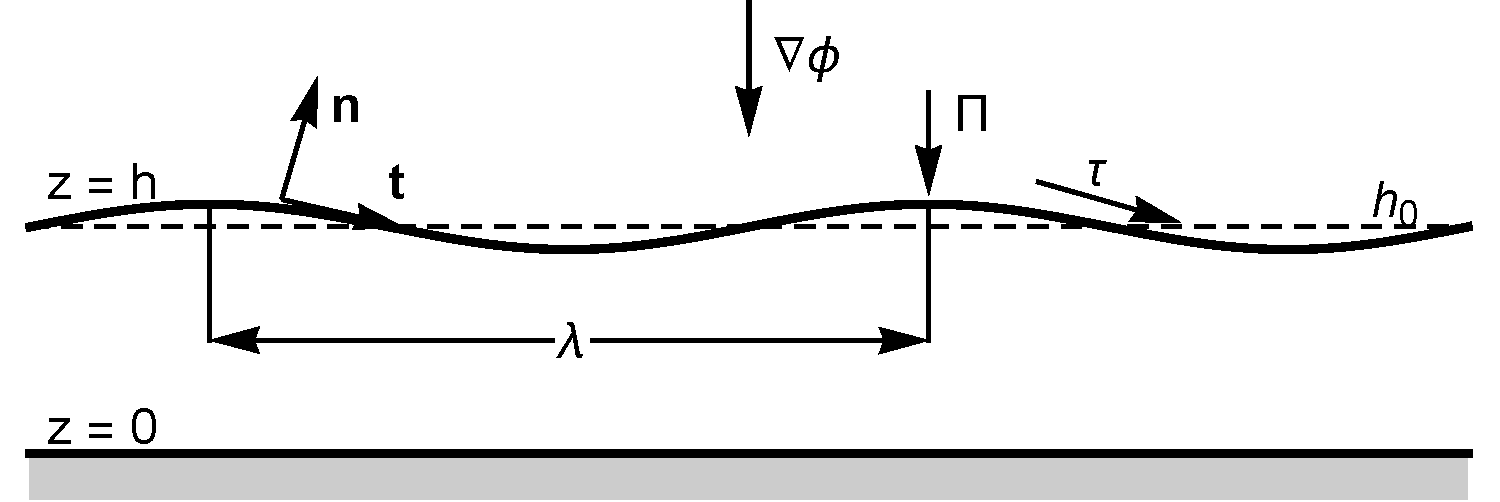
\includegraphics[scale=0.45]{figures/ThinFilm.pdf}
    \caption{A diagram of the situation in question.}\label{fig:thin_film}
  \end{figure}

  These equations completely describe the fluid, but we are now going to make a
  lubrication approximation, through a scaling argument.
  For the lubrication approximation we are going to assume that the average height of
  the liquid, \(h_0\), is much smaller then the characterstic wavelength of the liquid,
  \(\lambda \).
  We will denote the ratio of these two lengths as \(\varepsilon \), that is
  \begin{equation}
    \varepsilon = \frac{h_0}{\lambda} \ll 1.
  \end{equation}
  Now we nondimensionalize the rest of the variables with respect to this ratio.
  We denote the nondimensional variables as the uppercase variables.
  As we stated earlier the characteristic height is \(h_0\) and the characteristic
  length is \(\lambda = h_0/\varepsilon \), so the nondimensional length variables are
  \begin{equation}
    Z = \frac{z}{h_0}, \quad X = \frac{\varepsilon x}{h_0}, \quad H = \frac{h}{h_0}.
  \end{equation}
  Let \(U_0\) be the characteristic horizontal velocity, then
  \begin{equation}
    \quad U = \frac{u}{U_0}, \quad W = \frac{w}{\varepsilon U_0}
  \end{equation}
  where the nondimensional vertical velocity, \(W\), follows from the continuity
  equation, equation~\eqref{eq:incompressibility}.
  It follows that time will be scaled by \(\lambda/U_0\), so nondimensional time is
  \begin{equation}
    T = \frac{\varepsilon U_0 t}{h_0}.
  \end{equation}
  Finally we assume that the flow is locally parallel or equivalently
  \(p_x \sim \mu u_{zz}\).
  This gives us the proper scaling for the pressure, gravity, and surface stresses,
  \begin{equation}
    P = \frac{\varepsilon h_0}{\mu U_0} p, \quad
    \Phi = \frac{\varepsilon h_0}{\mu U_0}\phi, \quad
    \Pi = \frac{\varepsilon h_0}{\mu U_0}\Pi_0, \quad
    \tau = \frac{h_0}{\mu U_0}\tau_0.
  \end{equation}
  Lastly we can nondimensionalize the surface tension as
  \begin{equation}
    \Sigma = \frac{\varepsilon \sigma}{\mu U_0}
  \end{equation}

  The following give some intermediate steps in how to nondimensionalize variables
  that include derivatives.
  \begin{align*}
    u_x &= U_0 U_X \pd{X}{x} = \frac{\varepsilon U_0}{h_0} U_X\\
    w_z &= \varepsilon U_0 W_Z \pd{Z}{z} = \frac{\varepsilon U_0}{h_0} W_Z \\
    u_t &= U_0 U_T \pd{T}{t} = \frac{\varepsilon U_0^2}{h_0} U_T \\
    uu_x &= U_0 U U_0 U_X \pd{X}{x} = \frac{\varepsilon U_0^2}{h_0} UU_X \\
    wu_z &= \varepsilon U_0 W U_0 U_Z \pd{Z}{z} = \frac{\varepsilon U_0^2}{h_0} WU_Z \\
    w_t &= \varepsilon U_0 W_T \pd{T}{t} = \frac{\varepsilon^2 U_0^2}{h_0} W_T \\
    uw_x &= U_0 U \varepsilon U_0 W_X \pd{X}{x} = \frac{\varepsilon^2 U_0^2}{h_0} UW_X \\
    ww_z &= \varepsilon U_0 W \varepsilon U_0 W_Z \pd{Z}{z} = \frac{\varepsilon^2 U_0^2}{h_0} WW_Z \\
    p_x &= \frac{\mu U_0}{\varepsilon h_0} P_X \pd{X}{x} = \frac{\mu U_0}{h_0^2} P_X \\
    p_z &= \frac{\mu U_0}{\varepsilon h_0} P_Z \pd{Z}{z} = \frac{\mu U_0}{\varepsilon h_0^2} P_Z \\
    u_{xx} &= U_0 U_{XX} \p{\pd{X}{x}}^2 = \frac{\varepsilon^2 U_0}{h_0^2} U_{XX} \\
    u_{zz} &= U_0 U_{ZZ} \p{\pd{Z}{z}}^2 = \frac{U_0}{h_0^2} U_{ZZ} \\
    w_{xx} &= \varepsilon U_0 W_{XX} \p{\pd{X}{x}}^2 = \frac{\varepsilon^3 U_0}{h_0^2} W_{XX} \\
    w_{zz} &= \varepsilon U_0 U_{ZZ} \p{\pd{Z}{z}}^2 = \frac{\varepsilon U_0}{h_0^2} W_{ZZ} \\
    \phi_x &= \frac{\mu U_0}{\varepsilon h_0} \Phi_X \pd{X}{x} = \frac{\mu U_0}{h_0^2} \Phi_X \\
    \phi_z &= \frac{\mu U_0}{\varepsilon h_0} \Phi_Z \pd{Z}{z} = \frac{\mu U_0}{\varepsilon h_0^2} \Phi_Z \\
    h_t &= h_0 H_T \pd{T}{t} = \varepsilon U_0 H_T \\
    u h_x &= U_0 U h_0 H_X \pd{X}{x} = \varepsilon U_0 U H_X
  \end{align*}

  Substituting these nondimensional variables into the continuity
  equation~\eqref{eq:incompressibility}, gives
  \begin{align*}
    u_x + w_z &= 0 \\
    \frac{\varepsilon U_0}{h_0} U_X + \frac{\varepsilon U_0}{h_0} W_Z &= 0 \\
    U_X + W_Z &= 0
  \end{align*}
  This computation also justifies the scaling of \(w\) as the nondimensional variables
  should also conserve mass.

  We can nondimensionalize the conservation of momementum equations as follows,
  \begin{align*}
    \rho\p{u_t + u u_x + w u_z} &= -p_x + \mu \Delta u - \phi_x \\
    \rho\p{\frac{\varepsilon U_0^2}{h_0} U_T + \frac{\varepsilon U_0^2}{h_0} UU_X
    + \frac{\varepsilon U_0^2}{h_0} WU_Z} &= -\frac{\mu U_0}{h_0^2} P_X
    + \mu \p{\frac{\varepsilon^2 U_0}{h_0^2} U_{XX} + \frac{U_0}{h_0^2} U_{ZZ}}
    - \frac{\mu U_0}{h_0^2} \Phi_X \\
    \frac{\varepsilon U_0^2 \rho}{h_0}\p{U_T + UU_X + WU_Z} &=
    \frac{\mu U_0}{h_0^2}\p{-P_X + \p{\varepsilon^2 U_{XX} + U_{ZZ}} - \Phi_X } \\
    \frac{\varepsilon U_0 \rho h_0}{\mu}\p{U_T + UU_X + WU_Z} &=
    \p{-P_X + \p{\varepsilon^2 U_{XX} + U_{ZZ}} - \Phi_X }
  \end{align*}
  and
  \begin{align*}
    \rho\p{w_t + u w_x + w w_z} &= -p_z + \mu \Delta w - \phi_z \\
    \rho\p{\frac{\varepsilon^2 U_0^2}{h_0} W_T + \frac{\varepsilon^2 U_0^2}{h_0} UW_X
    + \frac{\varepsilon^2 U_0^2}{h_0} WW_Z} &= -\frac{\mu U_0}{\varepsilon h_0^2} P_Z
    + \mu \p{\frac{\varepsilon^3 U_0}{h_0^2} W_{XX}
    + \frac{\varepsilon U_0}{h_0^2} W_{ZZ}}
    - \frac{\mu U_0}{\varepsilon h_0^2} \Phi_Z \\
    \frac{\varepsilon^2 \rho U_0^2}{h_0}\p{W_T + UW_X + WW_Z} &=
    \frac{\mu U_0}{\varepsilon h_0^2} \p{-P_Z
    + \p{\varepsilon^4 W_{XX} + \varepsilon^2 W_{ZZ}} - \Phi_Z} \\
    \varepsilon^3 \frac{\rho U_0 h_0}{\mu}\p{W_T + UW_X + WW_Z} &=
    \p{-P_Z + \varepsilon^2\p{\varepsilon^2 W_{XX} + W_{ZZ}} - \Phi_Z}
  \end{align*}

  The boundary conditions are nondimensionalized as below,
  \begin{align*}
    w &= 0, u = 0 &\text{at } z = 0 \\
    \varepsilon U_0 W &= 0, U_0 U = 0 &\text{at } Z = 0 \\
    W &= 0, U = 0 &\text{at } Z = 0
  \end{align*}
  with
  \begin{align*}
    w &= h_t + u h_x &\text{at } z = h \\
    \varepsilon U_0 W &= \varepsilon U_0 H_T + \varepsilon U_0 U H_x &\text{at } Z = H \\
    W &= H_T + U H_x &\text{at } Z = H
  \end{align*}

  In order to nondimensionalize the stress tensor at the free surface, we consider the
  normal and tangential components of \(\v{T} \cdot \v{n}\) separately.
  The normal and tangential vector at the surface can be expressed in terms of the free
  surface as
  \begin{gather}
    \v{n} = \frac{\abr{-h_x, 1}}{\p{1 + h_x^2}^{1/2}} \quad
    \v{t} = \frac{\abr{1, h_x}}{\p{1 + h_x^2}^{1/2}}
  \end{gather}
  and the mean curvature, \(\kappa \), can be expressed in terms of \(h\) as
  \begin{equation}
    \kappa = -\frac{h_{xx}}{\p{1 + h_x^2}^{3/2}}.
  \end{equation}
  We would now like to write the following vector equation in terms of its normal and
  tangential components.
  \begin{align*}
    \v{T} \cdot \v{n} &= \p{-\kappa \sigma + \Pi_0}\v{n}
      + \p{\pd{\sigma}{s} + \tau_0}\v{t} &\text{at } z = h
  \end{align*}

  Note that we are using a Newtonian stress tensor which is given by
  \begin{align}
    \v{T} &=
    \begin{bmatrix}
      -p & 0 \\
      0 & -p
    \end{bmatrix} +
    \mu \begin{bmatrix}
      2u_x & u_z + w_x \\
      u_z + w_x & 2w_z
    \end{bmatrix}
  \end{align}

  The normal component of this vector equation is given by
  \begin{align}
    \abr{\v{T} \cdot \v{n}, \v{n}} &= \p{-\kappa \sigma + \Pi_0}
  \end{align}

  First we will simplify the left hand side.
  \begin{align*}
    a &= \p{1 + h_x^2}^{1/2} \\
    \abr{\v{T} \cdot \v{n}, \v{n}} &= \frac{1}{a^2}
    \begin{bmatrix}
      -h_x & 1
    \end{bmatrix}
    \begin{bmatrix}
      -p + 2 \mu u_x & \mu \p{u_z + w_x} \\
      \mu \p{u_z + w_x} & -p + 2 \mu w_z
    \end{bmatrix}
    \begin{bmatrix}
      -h_x \\
      1
    \end{bmatrix} \\
    &=
    \frac{1}{a^2}
    \begin{bmatrix}
      -h_x & 1
    \end{bmatrix}
    \begin{bmatrix}
      -h_x \p{-p + 2 \mu u_x} + \mu \p{u_z + w_x} \\
      -h_x \mu \p{u_z + w_x} + -p + 2\mu w_z
    \end{bmatrix} \\
    &= \frac{1}{a^2} \p{h_x^2\p{-p + 2\mu u_x} - \mu h_x \p{u_z + w_x}
      - \mu h_x \p{u_z + w_x} + -p + 2\mu w_z} \\
    &= \frac{1}{a^2} \p{h_x^2\p{-p + 2 \mu u_x}
      - 2 \mu h_x \p{u_z + w_x} - p + 2\mu w_z} \\
    &= \frac{1}{a^2} \p{\p{1 + h_x^2} \p{-p} + 2 \mu \p{h_x^2 u_x + w_z}
      - 2 \mu h_x \p{u_z + w_x}} \\
    &= -p + \frac{2 \mu}{a^2} \p{\p{h_x^2 u_x + w_z}
      - h_x \p{u_z + w_x}}
  \end{align*}
  Next simplify the right hand side.
  \begin{align*}
    \p{-\kappa \sigma + \Pi_0} &= \frac{h_{xx}}{\p{1 + h_x^2}^{3/2}} \sigma + \Pi_0
  \end{align*}
  This gives the following scalar equation,
  \begin{align}
    -p - \Pi_0 + \frac{2 \mu}{1 + h_x^2} \p{\p{h_x^2 u_x + w_z}
      - h_x \p{u_z + w_x}} &= \frac{h_{xx}}{\p{1 + h_x^2}^{3/2}} \sigma.
  \end{align}

  The tangential component is given by
  \begin{align}
    \abr{\v{T} \cdot \v{n}, \v{t}} &= \p{\pd{\sigma}{s} + \tau_0}
  \end{align}
  First simplify the left hand side,
  \begin{align*}
    \abr{\v{T} \cdot \v{n}, \v{n}} &= \frac{1}{a^2}
    \begin{bmatrix}
      1 & h_x
    \end{bmatrix}
    \begin{bmatrix}
      -p + 2 \mu u_x & \mu \p{u_z + w_x} \\
      \mu \p{u_z + w_x} & -p + 2 \mu w_z
    \end{bmatrix}
    \begin{bmatrix}
      -h_x \\
      1
    \end{bmatrix} \\
    &=
    \frac{1}{a^2}
    \begin{bmatrix}
      1 & h_x
    \end{bmatrix}
    \begin{bmatrix}
      -h_x \p{-p + 2 \mu u_x} + \mu \p{u_z + w_x} \\
      -h_x \mu \p{u_z + w_x} + -p + 2\mu w_z
    \end{bmatrix} \\
    &= \frac{1}{a^2} \p{-h_x \p{-p + 2 \mu u_x} + \mu \p{u_z + w_x}
      + -h_x^2 \mu \p{u_z + w_x} + h_x \p{-p + 2\mu w_z}} \\
    &= \frac{1}{a^2} \p{-h_x \p{2 \mu u_x} + \mu \p{u_z + w_x}
      + -h_x^2 \mu \p{u_z + w_x} + h_x \p{2\mu w_z}} \\
    &= \frac{\mu}{a^2} \p{2 h_x \p{w_z - u_x} + \p{1 - h_x^2} \p{u_z + w_x}}
  \end{align*}
  Next simplify the right hand side
  \begin{align*}
    \p{\pd{\sigma}{s} + \tau_0} &= \pd{\sigma}{x} \pd{x}{s} + \tau_0\\
    &= \pd{\sigma}{x} \frac{1}{\p{1 + h_x^2}^{1/2}} + \tau_0
  \end{align*}
  This gives the following scalar equation.
  \begin{align}
    \mu \p{2 h_x \p{w_z - u_x} + \p{1 - h_x^2} \p{u_z + w_x}} &= \pd{\sigma}{x} \p{1 + h_x^2}^{1/2} + \tau_0\p{1 + h_x^2}
  \end{align}

  Lastly we will nondimensionalize these two equations.
  \begin{gather*}
    -p - \pi + \frac{2 \mu}{1 + h_x^2} \p{\p{h_x^2 u_x + w_z}
      - h_x \p{u_z + w_x}} = \frac{h_{xx}}{\p{1 + h_x^2}^{3/2}} \sigma \\
    -\frac{\mu U_0}{\varepsilon h_0}P - \frac{\mu U_0}{\varepsilon h_0}\Pi + \frac{2 \mu}{1 + \varepsilon^2 H_X^2} \p{\p{\varepsilon^2 H_X^2 \frac{\varepsilon U_0}{h_0} U_X + \frac{\varepsilon U_0}{h_0} W_Z}
      - \varepsilon H_X \p{\frac{U_0}{h_0} U_Z + \frac{\varepsilon^2 U_0}{h_0} W_X}} \\
      = \frac{\varepsilon^2}{h_0}\frac{H_{XX}}{\p{1 + \varepsilon^2 H_X^2}^{3/2}} \frac{\mu U_0}{\varepsilon} \Sigma \\
    \p{-\frac{\mu U_0}{\varepsilon h_0}P - \frac{\mu U_0}{\varepsilon h_0}\Pi + \frac{\varepsilon \mu U_0}{h_0}\frac{2}{1 + \varepsilon^2 H_X^2} \p{\p{\varepsilon^2 H_X^2 U_X + W_Z}
      - H_X \p{U_Z + \varepsilon^2 W_X}}} \\
      = \frac{\varepsilon \mu U_0}{h_0}\frac{H_{XX}}{\p{1 + \varepsilon^2 H_X^2}^{3/2}} \Sigma \\
    \p{-\frac{\mu U_0}{\varepsilon h_0}P - \frac{\mu U_0}{\varepsilon h_0}\Pi + \frac{\varepsilon \mu U_0}{h_0}\frac{2}{1 + \varepsilon^2 H_X^2} \p{\p{\varepsilon^2 H_X^2 U_X + W_Z}
      - H_X \p{U_Z + \varepsilon^2 W_X}}} \\
      = \frac{\varepsilon \mu U_0}{h_0}\frac{H_{XX}}{\p{1 + \varepsilon^2 H_X^2}^{3/2}} \Sigma \\
    \frac{\mu U_0}{\varepsilon h_0}\p{-P - \Pi + \frac{2 \varepsilon^2}{1 + \varepsilon^2 H_X^2} \p{\p{\varepsilon^2 H_X^2 U_X + W_Z}
      - H_X \p{U_Z + \varepsilon^2 W_X}}}
      = \frac{\mu U_0}{\varepsilon h_0}\frac{\varepsilon^2 H_{XX}}{\p{1 + \varepsilon^2 H_X^2}^{3/2}} \Sigma \\
    \p{-P - \Pi + \frac{2 \varepsilon^2}{1 + \varepsilon^2 H_X^2} \p{\p{\varepsilon^2 H_X^2 U_X + W_Z}
      - H_X \p{U_Z + \varepsilon^2 W_X}}}
      = \frac{\varepsilon^2 H_{XX}}{\p{1 + \varepsilon^2 H_X^2}^{3/2}} \Sigma
  \end{gather*}
  and
  \begin{gather*}
    \mu \p{2 h_x \p{w_z - u_x} + \p{1 - h_x^2} \p{u_z + w_x}} = \pd{\sigma}{x} \p{1 + h_x^2}^{1/2} + \tau_0\p{1 + h_x^2} \\
    \mu \p{2 \varepsilon H_X \p{\frac{\varepsilon U_0}{h_0} W_Z - \frac{\varepsilon U_0}{h_0} U_X}
    + \p{1 - \varepsilon^2 H_X^2} \p{\frac{U_0}{h_0} U_Z + \frac{\varepsilon^2 U_0}{h_0} W_X}} \\
    = \frac{\mu U_0}{h_0} \Sigma_X \p{1 + \varepsilon^2 H_X^2}^{1/2}
    + \frac{\mu U_0}{h_0} \tau \p{1 + \varepsilon^2 H_X^2} \\
    \frac{\mu U_0}{h_0} \p{2 \varepsilon^2 H_X \p{W_Z - U_X}
    + \p{1 - \varepsilon^2 H_X^2} \p{U_Z + \varepsilon^2 W_X}} \\
    = \frac{\mu U_0}{h_0} \p{\Sigma_X \p{1 + \varepsilon^2 H_X^2}^{1/2}
    + \tau \p{1 + \varepsilon^2 H_X^2}} \\
    2 \varepsilon^2 H_X \p{W_Z - U_X} + \p{1 - \varepsilon^2 H_X^2} \p{U_Z + \varepsilon^2 W_X} \\
    = \Sigma_X \p{1 + \varepsilon^2 H_X^2}^{1/2} + \tau \p{1 + \varepsilon^2 H_X^2}
  \end{gather*}

  The full nondimensional equations are thus
  \begin{align}
    U_X + W_Z &= 0 \\
    \frac{\varepsilon U_0 \rho h_0}{\mu}\p{U_T + UU_X + WU_Z} &=
    -P_X + \p{\varepsilon^2 U_{XX} + U_{ZZ}} - \Phi_X  \\
    \varepsilon^3 \frac{\rho U_0 h_0}{\mu}\p{W_T + UW_X + WW_Z} &=
    -P_Z + \varepsilon^2\p{\varepsilon^2 W_{XX} + W_{ZZ}} - \Phi_Z
  \end{align}
  at \(Z = 0\)
  \begin{gather}
    W = 0, \quad U = 0
  \end{gather}
  and at \(Z = H\)
  \begin{gather}
    W = H_T + U H_x \\
    -P - \Pi + \frac{2 \varepsilon^2}{1 + \varepsilon^2 H_X^2} \p{\p{\varepsilon^2 H_X^2 U_X + W_Z}
    - H_X \p{U_Z + \varepsilon^2 W_X}} = \frac{\varepsilon^2 H_{XX}}{\p{1 + \varepsilon^2 H_X^2}^{3/2}} \Sigma \\
    2 \varepsilon^2 H_X \p{W_Z - U_X} + \p{1 - \varepsilon^2 H_X^2} \p{U_Z + \varepsilon^2 W_X}
    = \Sigma_X \p{1 + \varepsilon^2 H_X^2}^{1/2} + \tau \p{1 + \varepsilon^2 H_X^2}
  \end{gather}

  We can now let \(\varepsilon \to 0\) which results in
  \begin{align}
    U_X + W_Z &= 0 \\
    P_X + \Phi_X &= U_{ZZ} \\
    P_Z + \Phi_Z &= 0
  \end{align}
  at \(Z = 0\),
  \begin{gather}
    W = 0, \quad U = 0 \\
  \end{gather}
  and at \(Z = H\)
  \begin{align}
    W &= H_T + U H_x  \\
    -P - \Pi &= \bar{\Sigma} H_{XX} \\
    U_Z &= \Sigma_X + \tau
  \end{align}
  Note that we assume that the surface tension is large, so that
  \(\bar{\Sigma} = \varepsilon^2 \Sigma = O(1)\).
  This is important in order to keep surface tension effects in the final equation.

  Next we integrate the continuity equation over \(Z\).
  \begin{align*}
    \dintt{0}{H}{U_X + W_Z}{Z} &= 0 \\
    \dintt{0}{H}{U_X}{Z} + \eval*{W}{Z = 0}{H} &= 0 \\
    \dintt{0}{H}{U_X}{Z} + H_T + U H_X &= 0 \\
    H_T + \dintt{0}{H}{U_X}{Z} + U H_X &= 0 \\
    H_T + \pda{\dintt{0}{H}{U}{Z}}{X} &= 0
  \end{align*}

  Using the boundary conditions we can solve for an expression of \(U\) as follows
  \begin{align*}
    \dintt{Z}{H}{U_{ZZ}}{Z} &= \dintt{Z}{H}{P_X + \Phi_X}{Z} \\
    \eval*{U_Z}{Z}{H} &= \p{P_X + \Phi_X}\p{H - Z} \\
    \p{\tau + \Sigma_X} - U_Z &= \p{P_X + \Phi_X}\p{H - Z} \\
    \dintt{0}{Z}{\p{\tau + \Sigma_X} - U_Z}{Z} &= \dintt{0}{Z}{\p{P_X + \Phi_X}\p{H - Z}}{Z} \\
    \p{\tau + \Sigma_X}Z - \eval*{U}{Z = 0}{Z} &= \p{P_X + \Phi_X}\p{HZ - \frac{1}{2} Z^2} \\
    \p{\tau + \Sigma_X}Z - U &= \p{P_X + \Phi_X}\p{HZ - \frac{1}{2} Z^2} \\
    U &= \p{\tau + \Sigma_X}Z + \p{P_X + \Phi_X}\p{\frac{1}{2} Z^2 - HZ}
  \end{align*}

  The boundary conditions also give an expression for \(P + \Phi \),
  \begin{align*}
    P_Z + \Phi_Z &= 0 \\
    \dintt{Z}{H}{P_Z + \Phi_Z}{Z} &= 0 \\
    \eval{P}{Z=H} - P + \eval{\Phi}{Z=H} - \Phi &= 0 \\
    -\Pi - \bar{\Sigma} H_{XX} - P + \eval{\Phi}{Z=H} - \Phi &= 0 \\
    P + \Phi &= \eval{\Phi}{Z=H} - \Pi - \bar{\Sigma} H_{XX}
  \end{align*}

  Plugging both of these into the integrated continuity equation gives,
  \begin{align*}
    H_T + \pda{\dintt{0}{H}{U}{Z}}{X} &= 0 \\
    H_T + \pda{\dintt{0}{H}{\p{\tau + \Sigma_X}Z + \p{P_X + \Phi_X}\p{\frac{1}{2} Z^2 - HZ}}{Z}}{X} &= 0 \\
    H_T + \p{\frac{1}{2}\p{\tau + \Sigma_X}H^2 + \p{P_X + \Phi_X}\p{\frac{1}{6} H^3 - \frac{1}{2}H^3}}_X &= 0 \\
    H_T + \p{\frac{1}{2}\p{\tau + \Sigma_X}H^2 - \frac{1}{3}\p{P + \Phi}_X H^3}_X &= 0 \\
    H_T + \p{\frac{1}{2}\p{\tau + \Sigma_X}H^2 - \frac{1}{3}\p{\eval{\Phi}{Z=H} - \Pi - \bar{\Sigma} H_{XX}}_X H^3}_X &= 0 \\
    H_T + \p{\frac{1}{2}\p{\tau + \Sigma_X}H^2 - \frac{1}{3}\p{\eval{\Phi}{Z=H} - \Pi}_X H^3}_X &= - \p{\bar{\Sigma} H^3 H_{XXX}}_X
  \end{align*}

  This is our final Thin Film equation and taking all of the constants to be one gives
  \begin{equation}
    H_T + \p{H^2 - H^3}_X = - \p{H^3 H_{XXX}}_X
  \end{equation}
\end{document}